\section{Systemarchitektur}\label{sec:systemarchitektur}

Es gibt 3 große Services, das Chat Widget ~\ref{sec:chat-widget} auf der Schulhomepage, das Dashboard ~\ref{sec:dashboard} und das Backend ~\ref{sec:backend}.
Das System, das im Zuge der Arbeit entstand, sieht dabei folgendermaßen aus:

\begin{figure}[hbt!]
    \centering
    \includegraphics[scale=0.2]{pics/systemarchitektur}
    \caption{Systemarchitektur}
    \label{fig:impl:architektur}
\end{figure}

Es gibt zwei virtuelle Ubuntu Maschinen, nämlich eine für den Chat und eine für Rasa und das Backend.
Dadurch, dass der Chat auf die Seite der HTL Leonding Seite kommt, wird dadurch nur noch eine VM benötigt.

Der Chat wird dabei gerade mit NGINX gehostet.
Dieser Server kommuniziert mit Rasa direkt über REST, wenn die Benutzerin oder der Benutzer eine Nachricht sendet, wird diese an Rasa gesendet und Rasa antwortet mit der passenden Antwort.
Das Dashboard ~\ref{sec:dashboard} wird auf GH Pages gehostet, dieses kommuniziert mit dem Backend über REST.
Das Backend authentisiert sich dabei bei Rasa X ~\ref{subsec:rasa-x} und holt sich alle Konversationen.
Schließlich bereitet es die Konversationen auf und sendet sie an das Dashboard.

\section{Backend}\label{sec:backend}
\setauthor{Felix Dumfarth}

Das Quarkus ~\ref{quarkus} Backend hat die Aufgabe, mit Rasa X zu kommunizieren und die Konversationsdaten für das Dashboard aufzubereiten und zu senden.

Dieses Backend besitzt folgende Endpoints:

\begin{itemize}
    \item GET /api/conversations
    \item GET /api/conversations/{id}
    \item POST /api/feedback
    \item GET /api/feedback
    \item GET /api/file/{filename}
    \item PUT /api/file/{filename}
\end{itemize}

Bei den beiden \texttt{conversations} Endpoints muss man sich zunächst authentisieren und sich einen Bearer Token von Rasa x holen, damit auf die anderen Rasa X Endpoints zugegriffen werden kann.

\subsection{GET /api/conversations}
Der Endpoint ruft zuerst die getAuth() Funktion auf, um den Bearer Token zu erhalten.

Danach wird der Rasa X GET Endpoint ``/api/conversations'', mit dem Bearer Token im Header aufgerufen.
Von diesem Endpoint wird ein JSON Objekt zurückgegeben, das die Konversationen enthält, aber zusätzlich noch viele andere irrelevante Daten, deshalb filtert sich das Backend wirklich nur ID des Senders, die Zeit und die Anzahl von Nachrichten der Unterhaltungen heraus und gibt diese zurück.

\subsection{GET /api/conversations/{id}}
Der Endpoint \texttt{/api/conversations/{id}} ruft zuerst die \texttt{getAuth()} Funktion auf, um den Bearer Token zu erhalten.

Um nur die Nachrichten einer gezielten Unterhaltung zu erhalten, wird der Rasa X Endpoint \texttt{/api/conversations/{id}/messages}, mit dem Bearer Token im Header aufgerufen.
Die Response wird auch in dieser Form schon zurückgeben.

\subsection{POST /api/feedback}
Der Endpoint \texttt{/api/feedback} erhält ein JSON Objekt mit den Daten des Feedback-Formulars und speichert diese in die Datenbank.

\subsection{GET /api/feedback}
Der Endpoint \texttt{/api/feedback} liest alle Feedbacks aus der Datenbank aus und gibt diese zurück.

\subsection{GET /api/file/{filename}}
Der Endpoint \texttt{/api/file/{filename}} liest die im URL angegeben Datei aus dem Filesystem aus und gibt diese zurück.
Die möglichen Dateinamen sind:

\begin{itemize}
    \item nlu.yml
    \item rules.yml
    \item stories.yml
    \item config.yml
    \item domain.yml
\end{itemize}

\subsection{PUT /api/file/{filename}}
Der Endpoint \texttt{/api/file/{filename}} erhält den Inhalt aus dem File, welches auch im URL angegeben wurde und dieses dann im Filesystem überschreibt.

\section{Chat Widget}\label{sec:chat-widget}
Der Chatbot der HTL Leonding sollte auf der Schulhomepage als Chatblase angezeigt werden und verschiedene Elemente, wie Buttons und Links unterstützen.

\subsection{Konzept}
Während den Anfängen der vorliegenden Arbeit wurde ein Konzept erstellt, um das Design des Chatbots festzulegen.
Lange Zeit wurde der Chatbot, während der Entwicklung, unter dem Namen "Leon" geführt.
Dies wurde jedoch im späteren Verlauf geändert und "Leon" wurde Teil des langjährigen "Leonie Projektes" der HTL Leonding.

\begin{figure}[hbt!]
    \centering
    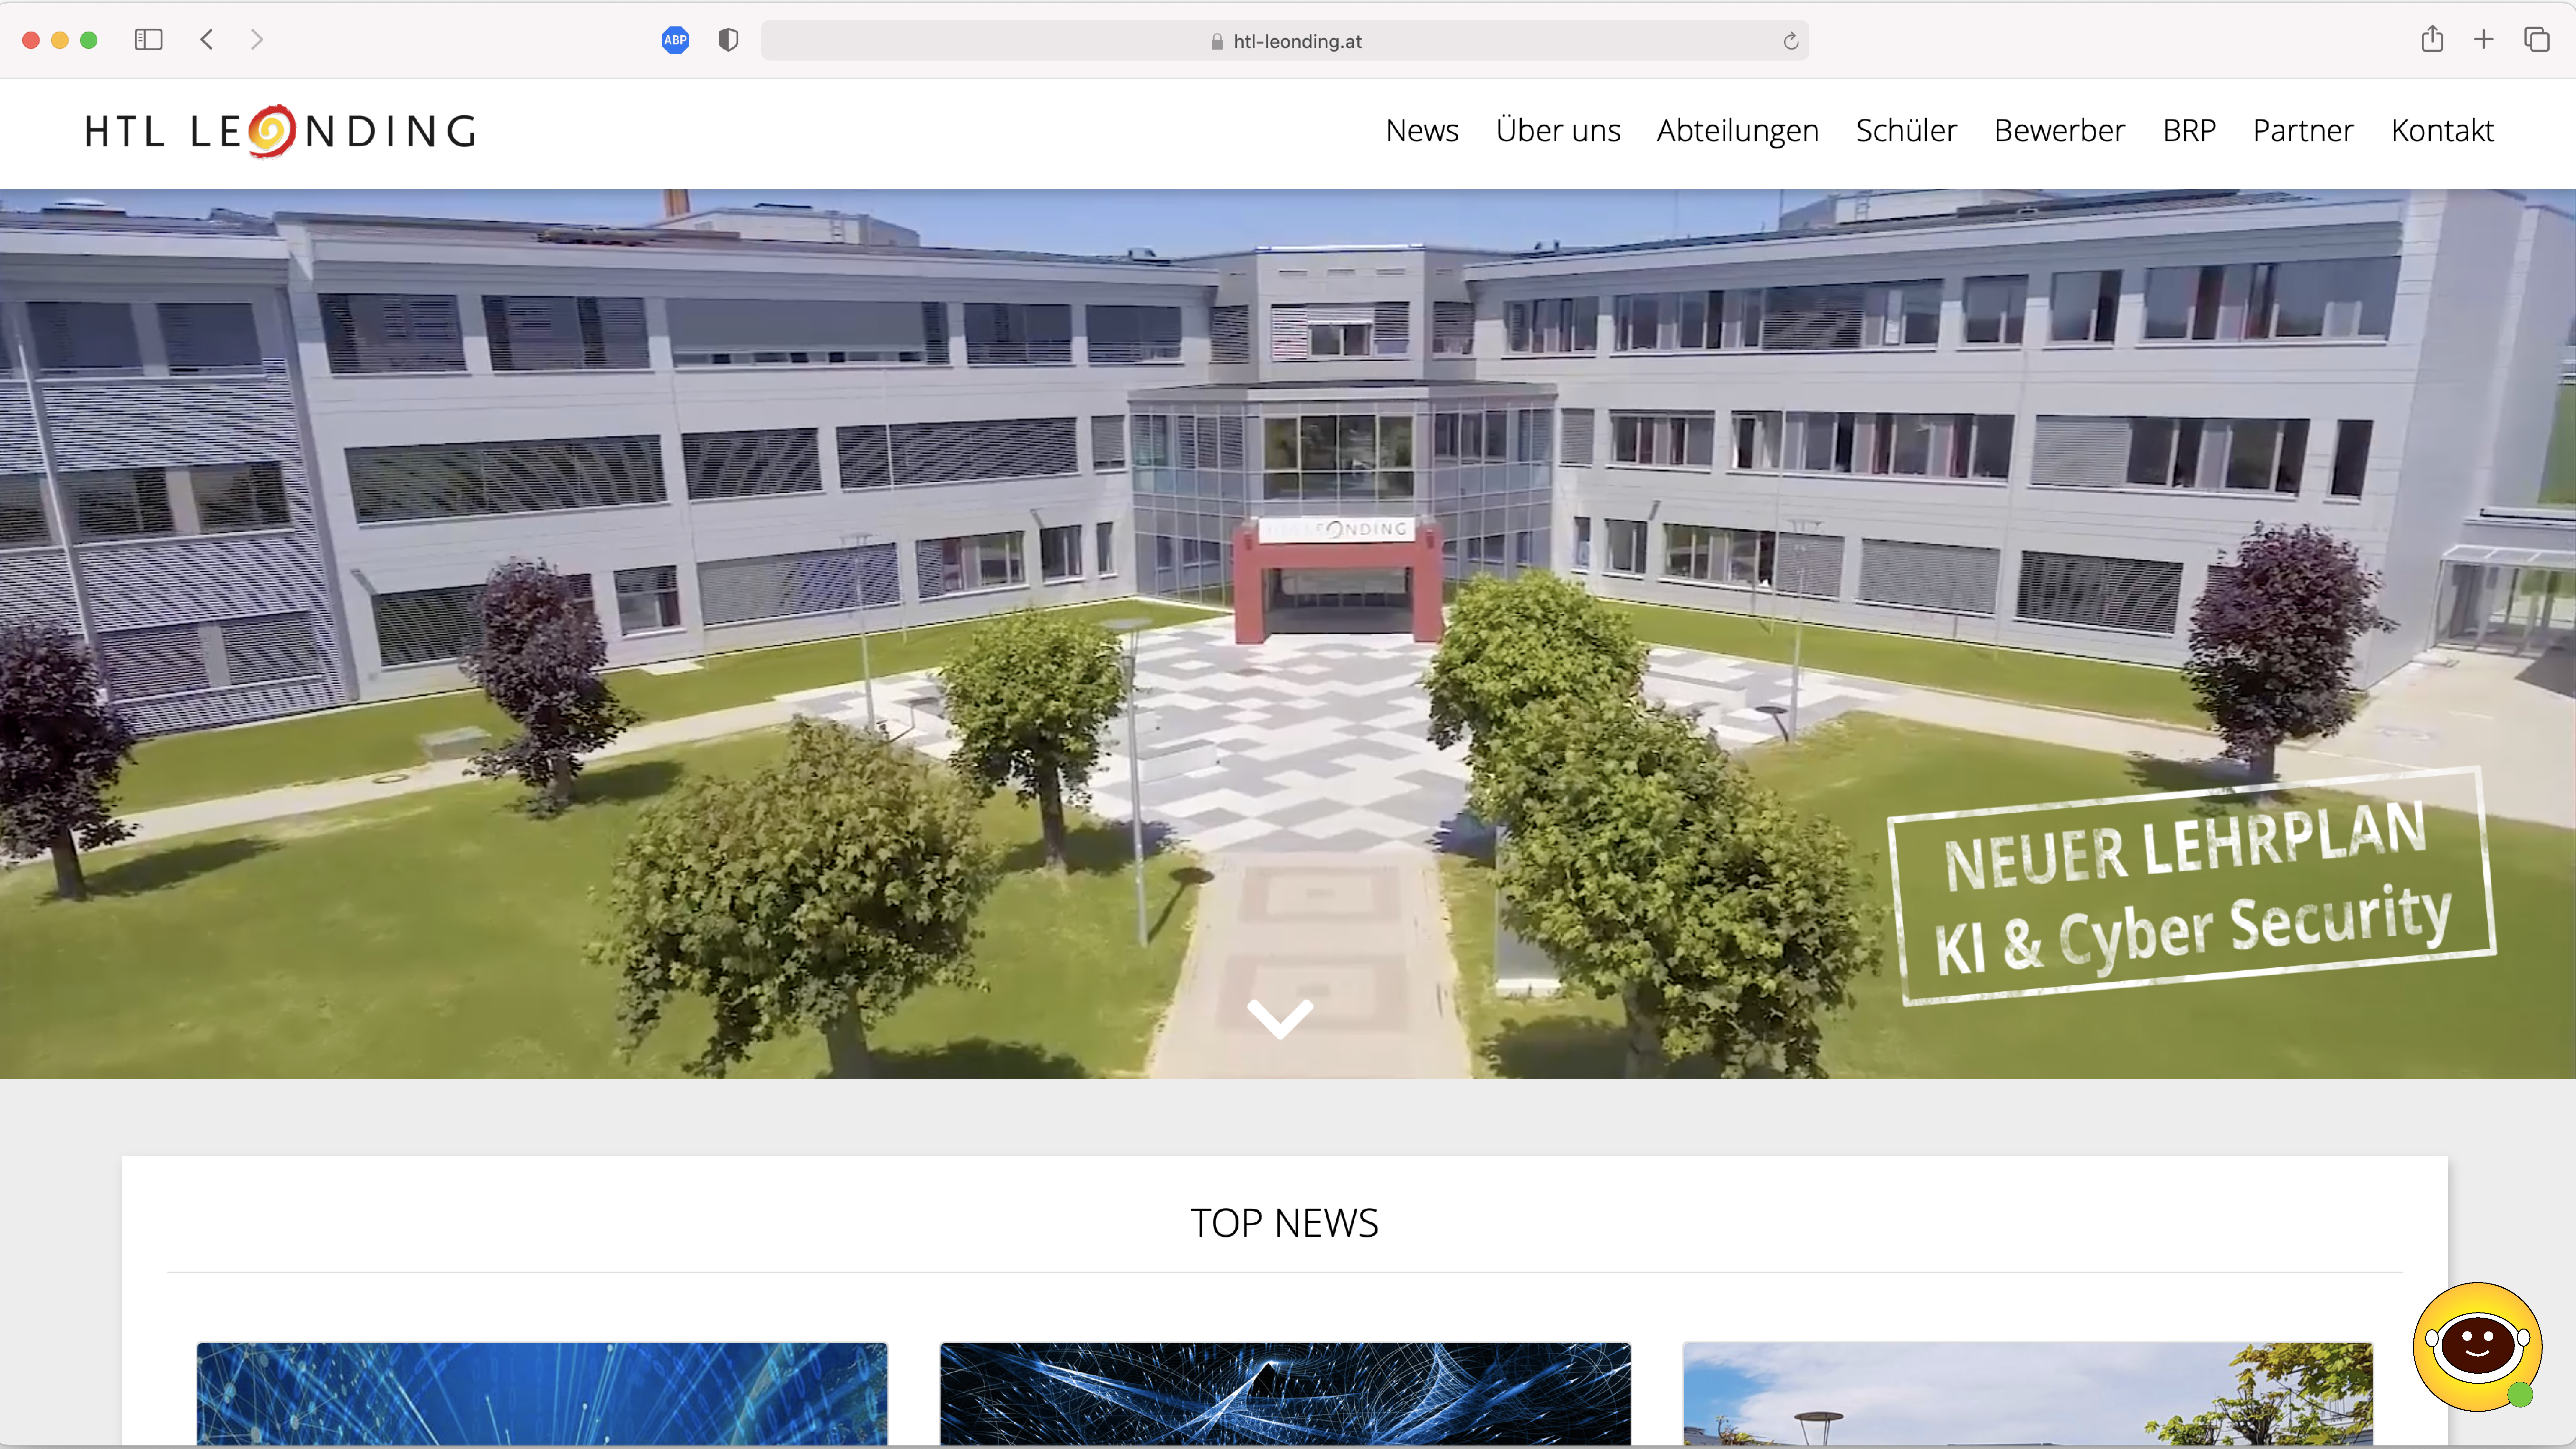
\includegraphics[scale=0.2]{pics/conceptBotClosed}
    \caption{Konzept Chatbot geschlossen}
    \label{fig:impl:conceptBotClosed}
\end{figure}
\begin{figure}[hbt!]
    \centering
    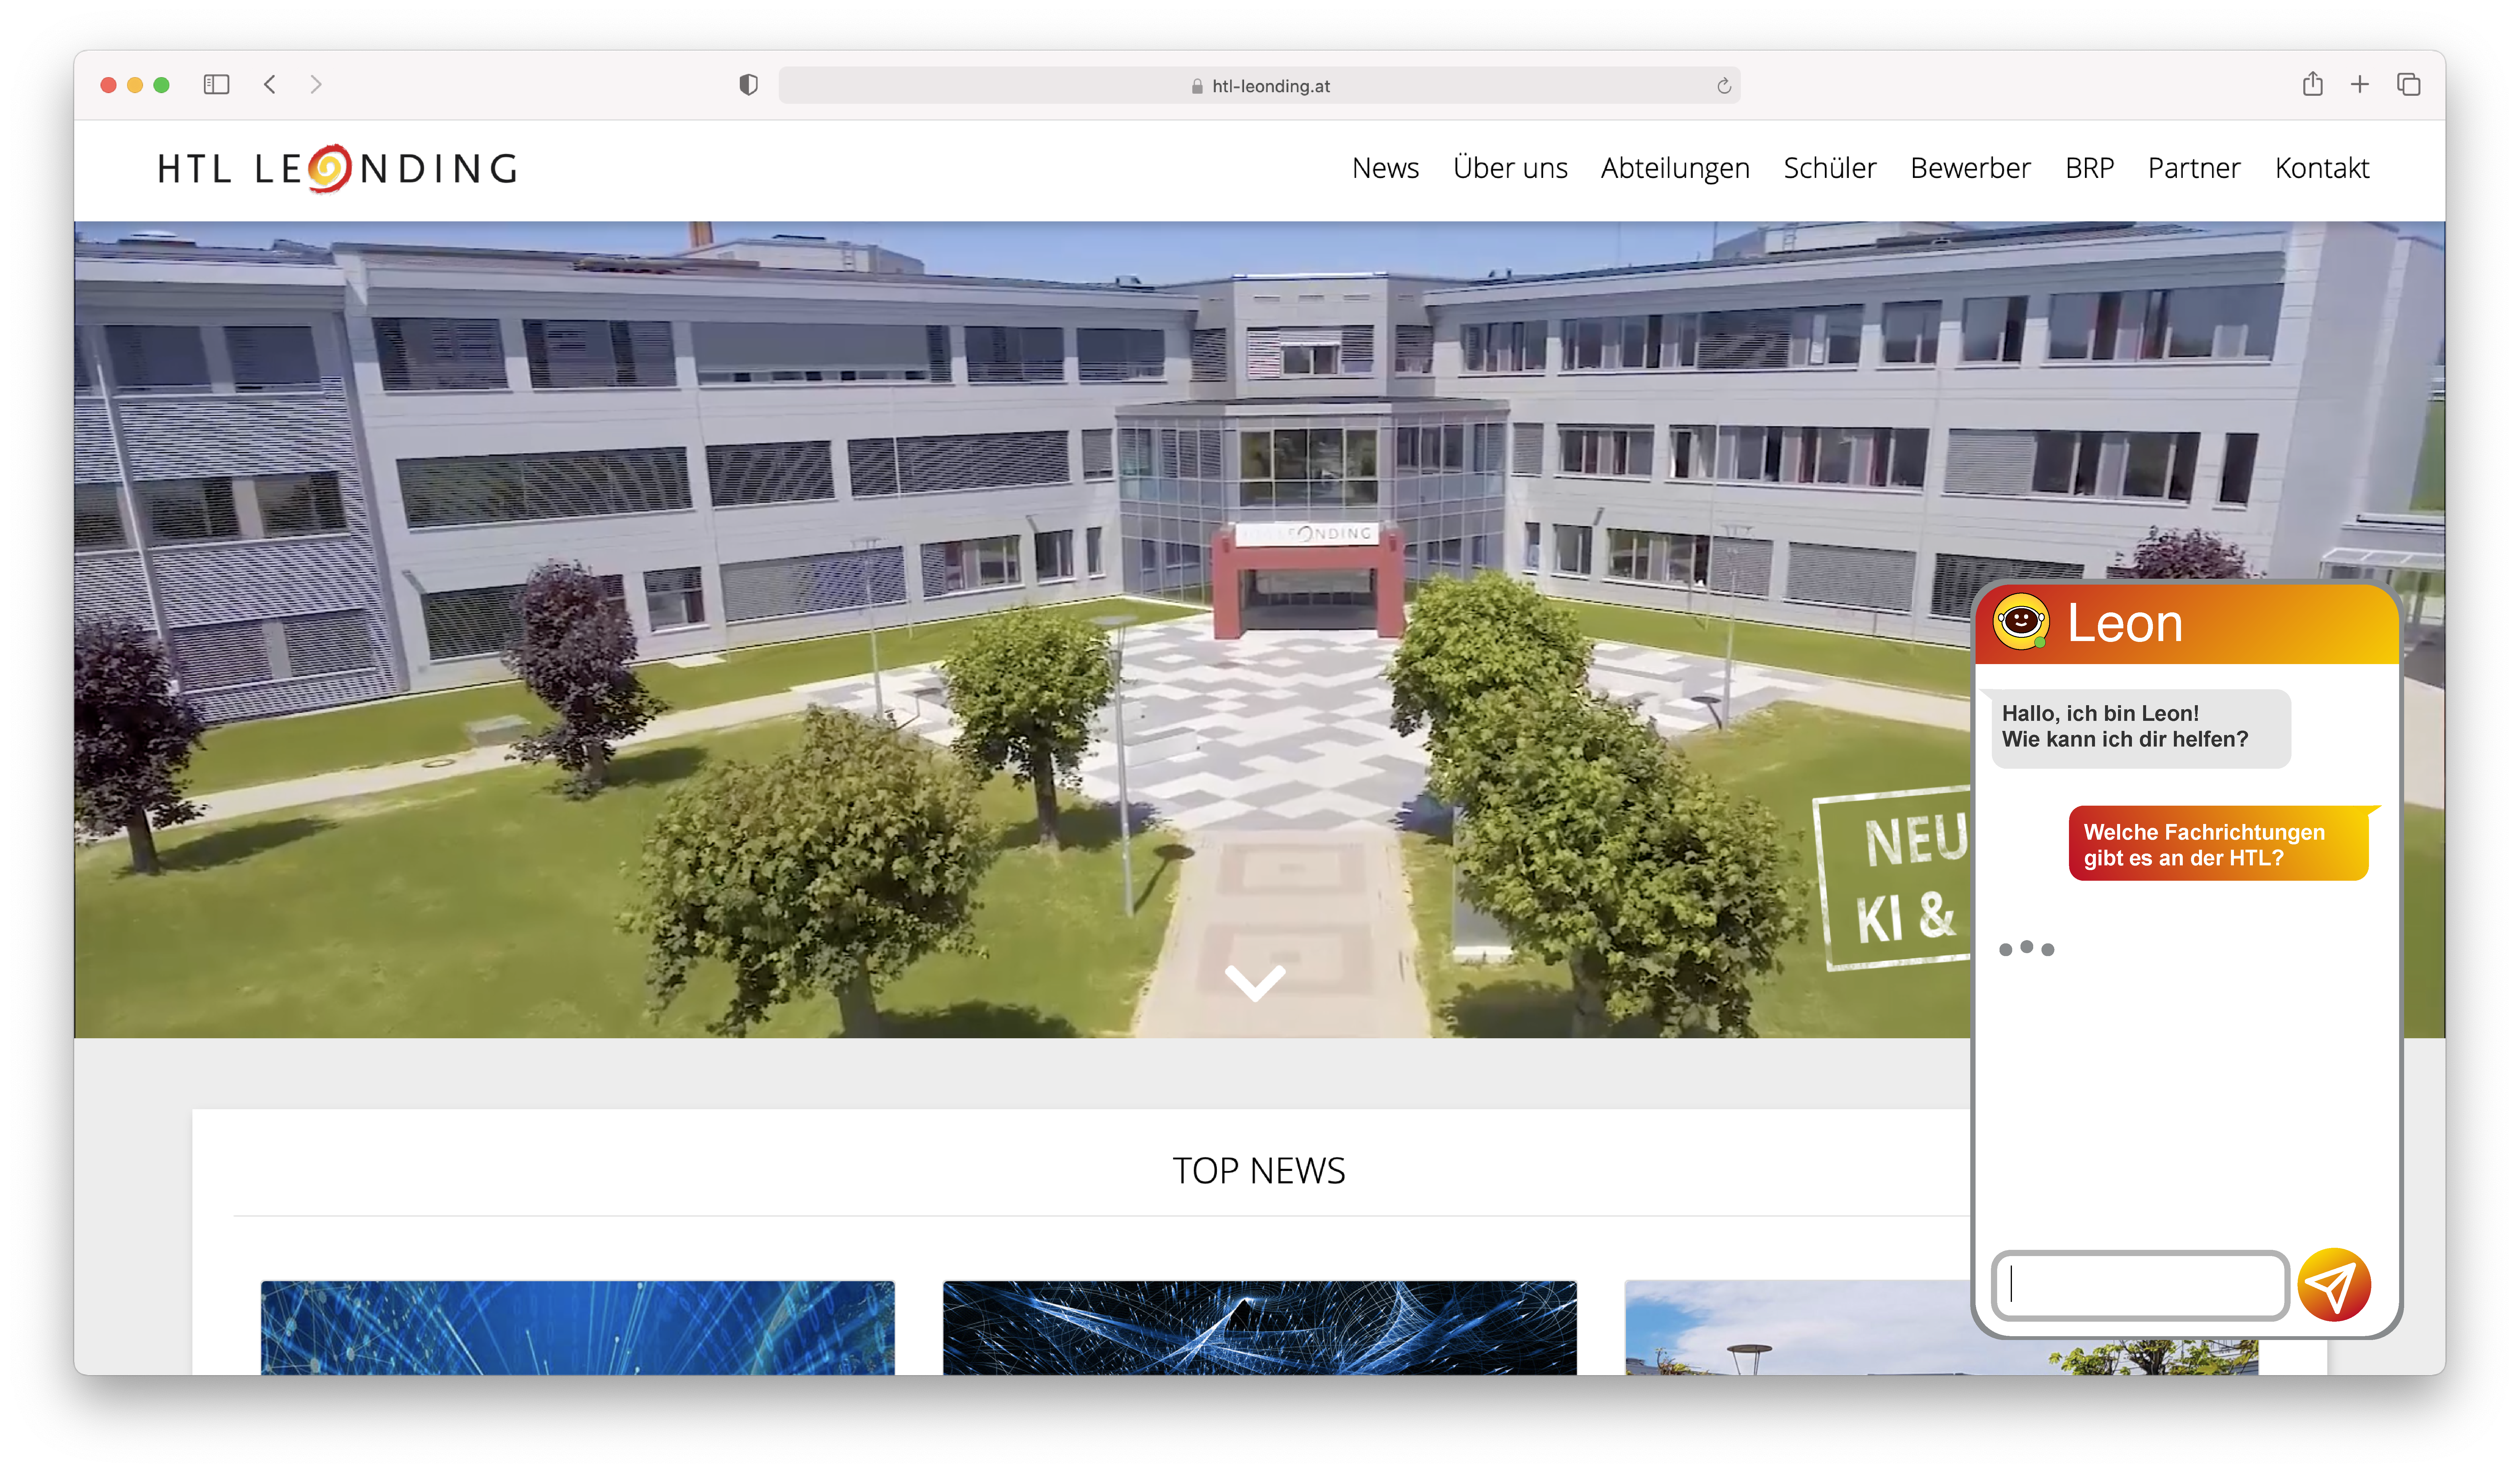
\includegraphics[scale=0.2]{pics/conceptBotOpen}
    \caption{Konzept Chatbot geöffnet}
    \label{fig:impl:conceptBotOpen}
\end{figure}

\subsection{Umsetzung}
Umgesetzt wurde das Frontend mithilfe von Angular.
Die Chatblase ist eine eigene Komponente, die durch CSS immer rechts unten fixiert ist.
Die Farben des Chatbots sollten dabei an die HTL Leonding erinnern, weshalb ein Farbverlauf aus Farben des HTL-Logos erstellt wurde.

Jedoch begann der Chatbot ganz anders und zu Beginn wurde der Bot als ganze Seite entwickelt und nicht nur als Chatblase.
Dies ist auf der Abbildung ~\ref{fig:impl:conceptBotFullPage} zu sehen.

\begin{figure}[hbt!]
    \centering
    \includegraphics[scale=0.2]{pics/fullPageBot}
    \caption{Chatbot auf einer ganzen Seite}
    \label{fig:impl:conceptBotFullPage}
\end{figure}

Dabei war dies nicht das endgültige Ziel und so kam es dazu, dass der Bot schnell zur Chatblase umgewandelt wurde.
Zum Testen war die HTL Leonding Seite mithilfe eines IFrames eingebunden und zusätzlich die Chatblasen Komponente.

Um das Gespräch in eine Richtung zu lenken, wurden Buttons eingeführt, die nach fast jeder Antwort mögliche Folgefragen vorschlagen.
Solche Vorschläge sind auf der Abbildung ~\ref{fig:impl:bot} zu sehen.

\begin{figure}[hbt!]
    \centering
    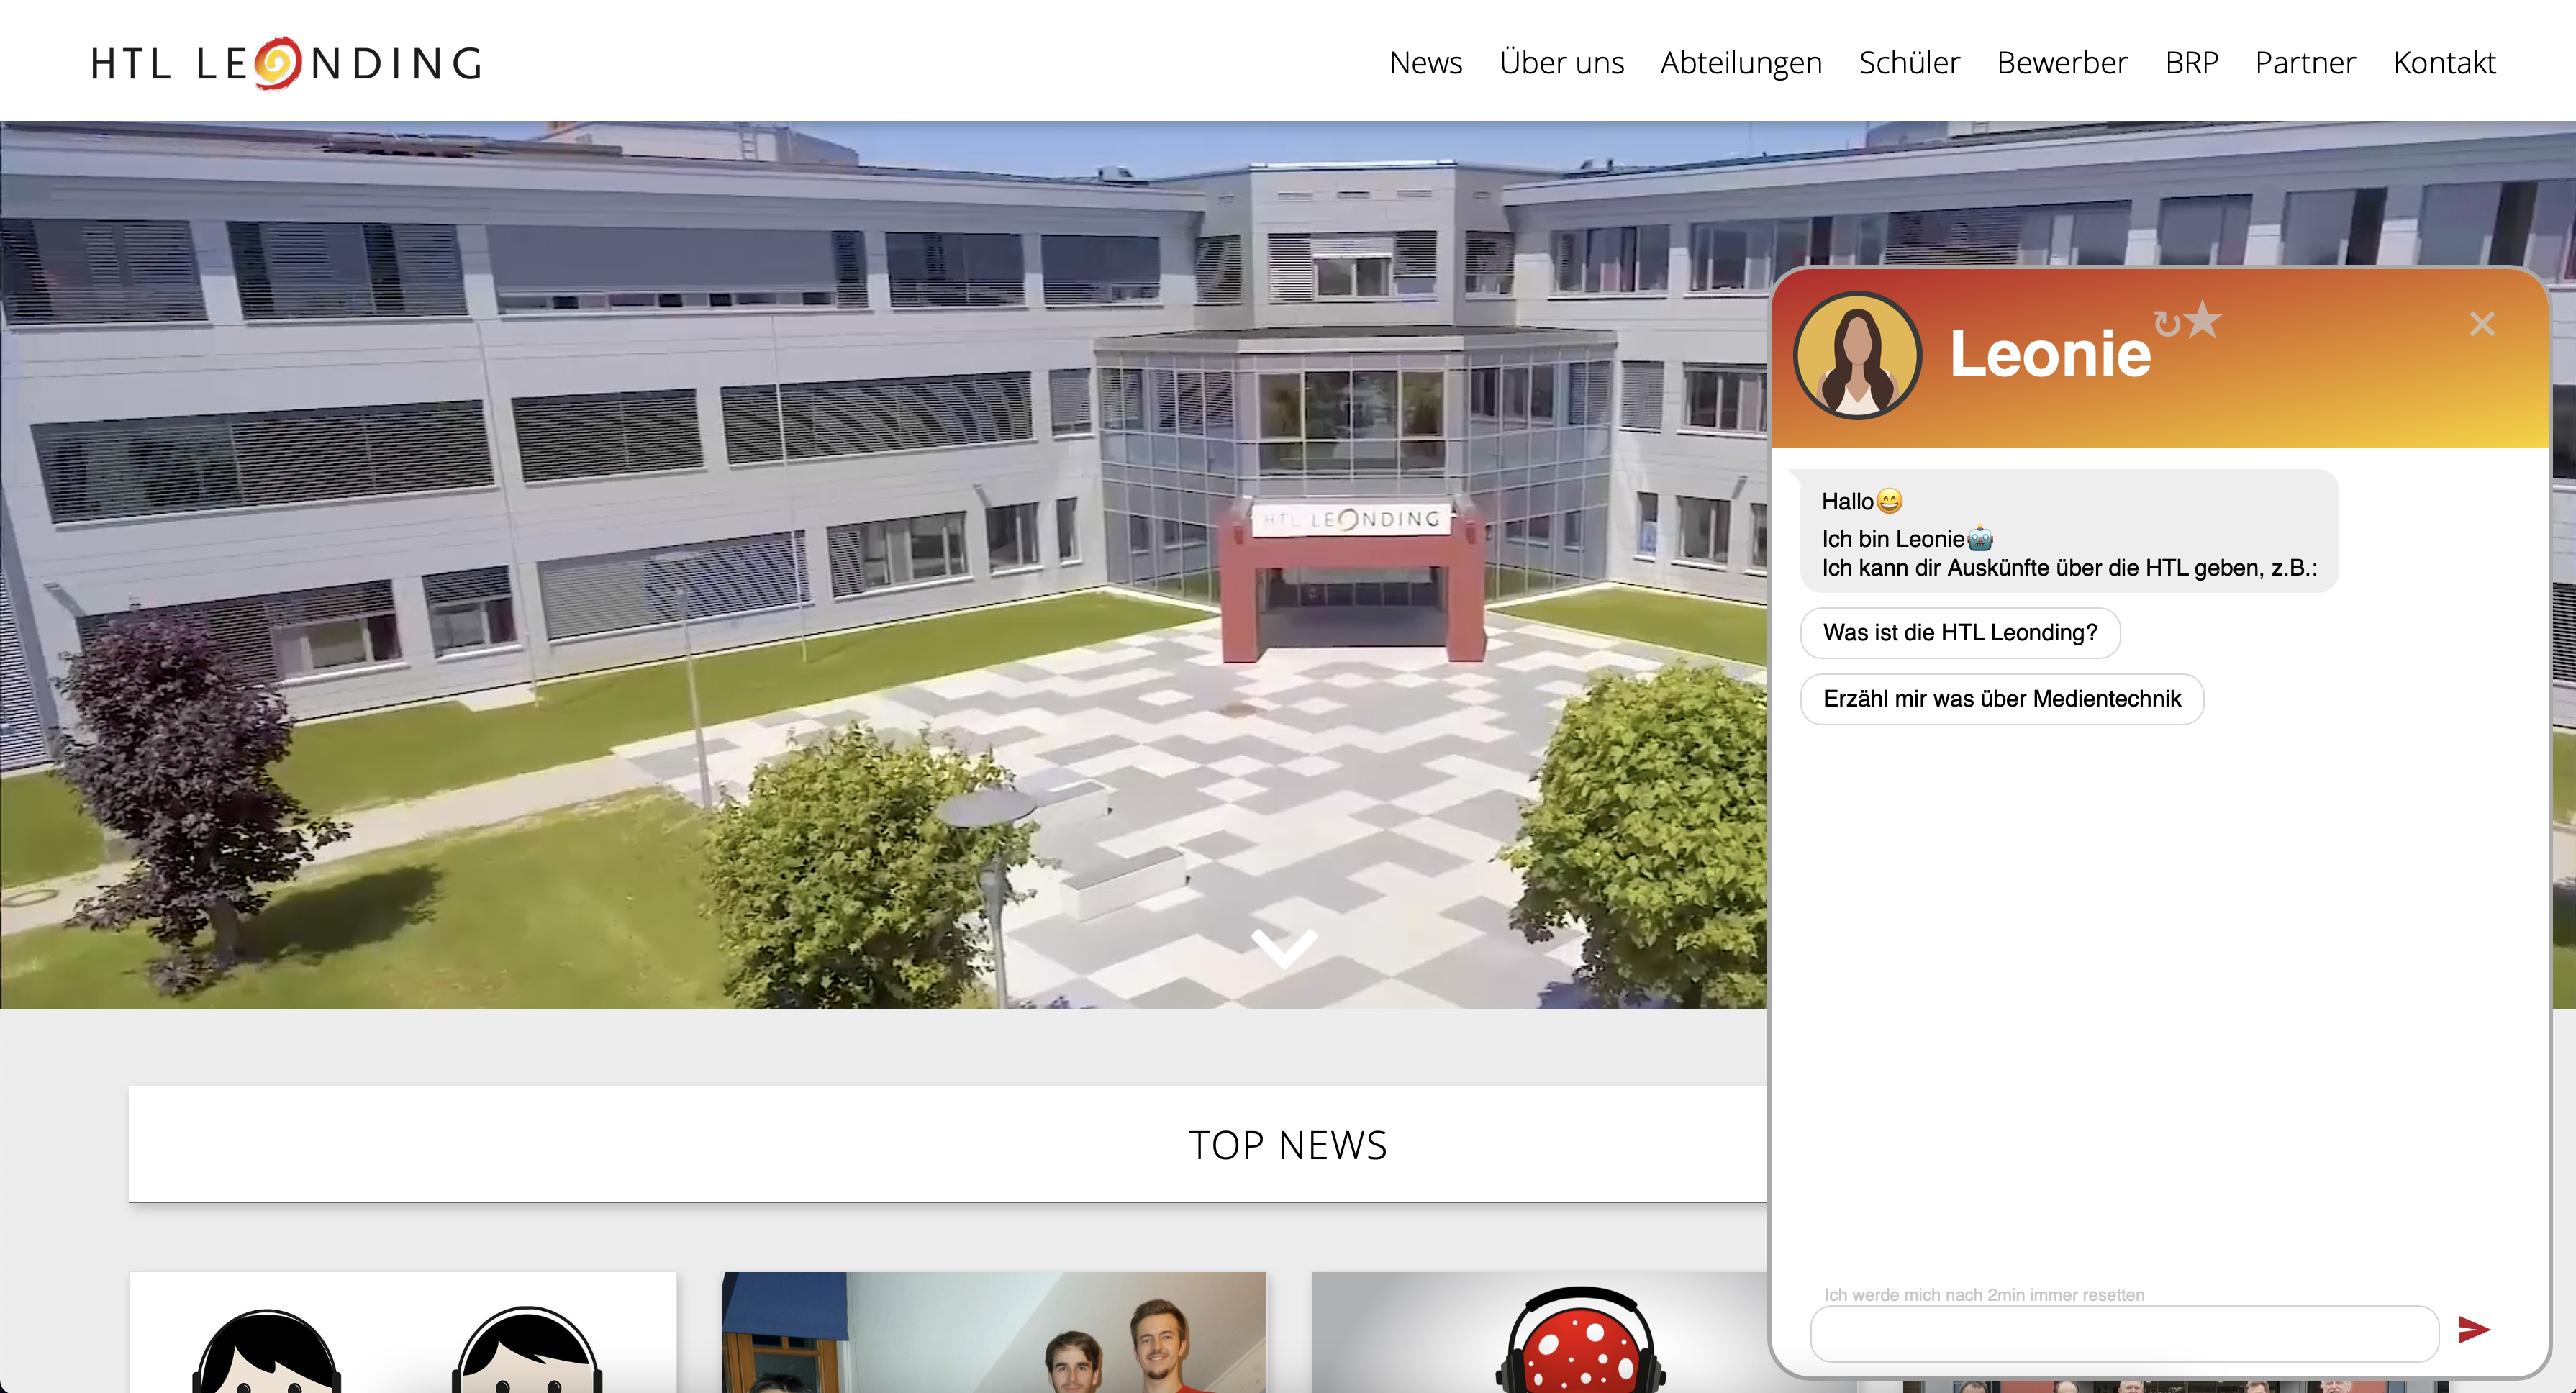
\includegraphics[scale=0.2]{pics/finalBot.png}
    \caption{Chatbot}
    \label{fig:impl:bot}
\end{figure}

Die Buttons werden von Rasa mit der Antwort auf die Frage mitgeschickt.
Wenn eine Benutzerin oder ein Benutzer auf einen der Buttons drückt, wird nicht der Text des Buttons an Rasa geschickt, sondern direkt die Bezeichnung des Intents mit einem ``/'' davor, da Rasa dies auch erkennt.

Um Bewertungen von echten Benutzern einzuholen, wurde außerdem eine Feedback-Seite eingeführt.
Auf dieser kann die Benutzerin oder der Benutzer eine Bewertung zwischen 1 und 5 Sternen abgeben und auch einen Text absenden.

\begin{figure}[hbt!]
    \centering
    \includegraphics[scale=0.3]{pics/feedback}
    \caption{Feedback Fenster}
    \label{fig:impl:feedback}
\end{figure}

Das Chatfenster wurde in wesentliche 3 Bereiche geteilt, die in Abbildung ~\ref{fig:impl:chatWidget} zu sehen sind.

\begin{figure}[hbt!]
    \centering
    \includegraphics[scale=0.4]{pics/chatWidgetStructure}
    \caption{Aufbau vom Chat Fenster}
    \label{fig:impl:chatWidget}
\end{figure}

\subsubsection{Avatar}
Wie bereits erwähnt, existiert der virtuelle Avatar der Leonie in Form einer 3D Pyramide und einer Website mit einem 3D Modell.
Um Verwirrung zu vermeiden, wurde entschieden, dass der Chatbot auch in ``Leonie'' umbenannt werden soll.
Bei der ursprünglichen Leonie handelt es sich um ein 3D Model (Abbildung ~\ref{fig:impl:leonie}).
Da dies aber nicht ganz zu einem Profilbild in einem Chat passen würde, wurde mit ``Adobe Illustrator'' eine 2D-Grafik erstellt.
Diese besteht aus einer färbigen Silhouette, welche die 3D-Leonie darstellt (Abbildung ~\ref{fig:impl:leonieTrans}).

\begin{figure}[hbt!]
    \centering
    \includegraphics[scale=0.5]{pics/AvatarLeonie}
    \caption{3D Leonie}
    \label{fig:impl:leonie}
\end{figure}

\begin{figure}[hbt!]
    \centering
    \includegraphics[scale=0.3]{pics/LeonieTrans}
    \caption{2D Leonie}
    \label{fig:impl:leonieTrans}
\end{figure}

\section{Dashboard}\label{sec:dashboard}
\setauthor{Felix Dumfarth}

Um alle Gespräche, sowie die Bewertungen der Benutzerinnen und Benutzer anzuzeigen, wurde ein Dashboard eingeführt, wo nur diese Funktionalitäten gegeben sind.
Im Laufe der Arbeit wurde dieses dann erweitert, um für den Leobot Conversation Cycle ~\ref{subsec:leobot-conversation-cycle} als Seite zu dienen.

\subsection{Conversation-Driven Development}\label{cdd}
\setauthor{Felix Dumfarth}

Rasa empfiehlt für die Entwicklung von Chatbots ``Conversation-Driven Development'', kurz CDD.\cite{cdd}
CDD beschreibt dabei eine Entwicklungsstrategie, in der der Chatbot nach Konversationen mit echten Usern verbessert wird.

Bei CDD wird empfohlen, dass man seinen Chatbot möglichst früh Personen zur Verfügung stehlt und so beobachten kann, welche Intents die echten Benutzerinnen und Benutzer erwarten und wie sie ihre Anfragen formulieren.
Als Entwicklerin oder Entwickler kann man diese nun bei Bedarf hinzufügen.


\subsection{Leobot Conversation Cycle}\label{subsec:leobot-conversation-cycle}
\setauthor{Felix Dumfarth}

\begin{figure}[hbt!]
    \centering
    \includegraphics[scale=0.2]{pics/LeoCircle}
    \caption{Leobot Conversation Cycle}
    \label{fig:impl:ConversationCycle}
\end{figure}

CDD ~\ref{cdd} wird mithilfe des Leobot Conversation Cycle umgesetzt.
Der Leobot Conversation Cycle ist ein Workflow, welcher dazu dient, den Leobot zu überprüfen und zu erweitern.
Der Workflow besteht dabei aus folgenden Schritten:

\begin{itemize}
    \item Unterhalten
    \item Überprüfen
    \item Verbessern
    \item Trainieren
\end{itemize}

Diese 4 Schritte werden immer wieder durchgeführt, um den Chatbot dauerhaft zu verbessern.

\subsubsection{Unterhalten}
Das Unterhalten ist der erste Schritt des Leobot Conversation Cycles.
In diesem Schritt werden dem Bot Fragen über die HTL Leonding und deren Produktangebot gestellt, die er anschließend beantworten soll.
Dies passiert während Unterhaltungen im Chat auf der Schulhomepage mit echten Personen.
Diese Unterhaltungen werden schließlich alle gespeichert.

\subsubsection{Überprüfen}

Das Überprüfen stellt den zweiten Schritt des Leobot Conversation Cycles dar.
In diesem Schritt wird vom Schulpersonal oder Verantwortlichen überprüft, ob der Bot die Fragen richtig beantwortet und erkannt hat oder ob Verbesserungspotenzial besteht

\subsubsection{Verbessern}
Das Verbessern ist der dritte Schritt des Leobot Conversation Cycles.
In diesem Schritt wird der Bot verbessert, das bedeutet, dass versucht wird, dass die Fehler verbessert werden.
Je nachdem, wo der Fehler des Bots liegt, muss hier anders gearbeitet werden.
Wenn es sich um einen eigentlich bekannten Intent handelt, jedoch die Formulierung des Benutzers nicht erkannt wurde, wird die Eingabe des Users zu den Trainingsdaten hinzugefügt.

Falls jemand aber eine Frage stellt, zu der es noch keinen passenden Intent gibt, so wird ein ganz neuer Intent zu den Trainingsdaten hinzugefügt.

\subsubsection{Trainieren}
Das Trainieren ist der vierte Schritt des Leobot Conversation Cycles.
In diesem Schritt werden die Trainingsdaten an den Bot übergeben und dieser wird trainiert.
Nachdem er fertig trainiert wurde, wechselt er auf das neu trainierte Model.

Und nun beginnt der Leobot Conversation Cycle wieder von vorne.

\subsubsection{Regelkreis}
\setauthor{Lukas Starka}

Dieser Vorgang erinnert dabei stark an einen Regelkreis.
Ein solcher Regelkreis ist in Abbildung ~\ref{fig:regelkreis} zu sehen und dieser führt eine Regelgröße auf einen gewünschten Sollwert.
Die Hauptkomponenten des Regelkreises sind der Regler und die Regelstrecke.
Beispielhaft ist die Regelstrecke ein Auto und die Fahrerin oder der Fahrer der Regler.
Dabei nimmt die Lenkerin oder der Lenker gewisse Parameter zur Hilfe, durch die entschieden wird, ob das Auto gelenkt, gebremst oder beschleunigt werden soll.
Diese Signale sind beispielsweise die aktuelle Geschwindigkeit, die Position des Autos oder die Fahrbahnverhältnisse.
Beim Regelkreis wird also eine Regelgröße über ein Eingangssignal der Regelstrecke zurückgeführt und auf einen gewünschten Wert gebracht.
Der Regelkreis wird oft bei der Regelung von Heizungen eingesetzt ~\ref{fig:heizungRegelKreis}.\cite{regelkreis, regelkreisBeispiel}

\begin{figure}[hbt!]
    \centering
    \includegraphics[scale=0.8]{pics/regelkreis}
    \caption{Allgemeiner Regelkreis ~\cite{regelkreis}}
    \label{fig:regelkreis}
\end{figure}

\begin{figure}[hbt!]
    \centering
    \includegraphics[scale=0.8]{pics/regelkreis_heizung}
    \caption{Regelkreis am Beispiel einer Heizung ~\cite{regelkreis}}
    \label{fig:heizungRegelKreis}
\end{figure}

Ein Regelkreis wird dabei entweder durch eine Änderung der Sollgröße oder durch Auftreten einer Störung ausgelöst.
Beim Leobot Conversation Cycle wird der Regelkreis demzufolge ausgelöst, wenn eine Interaktion mit einem User stattfand, bei der der Bot eine falsche Antwort gegeben hat.
Die Messeinrichtung ist dabei das Dashboard ~\ref{sec:dashboard}, das alle Unterhaltungen auflistet und diese grafisch veranschaulicht.
Durch den eingebauten Editor ist die Möglichkeit gegeben, dass direkt die Files bearbeitet werden, sodass der Bot in Zukunft auch auf diese Fragestellung die richtige Antwort parat hat.
Der Sollwert wird also in den Regler eingegeben und anschließend wird das Modell basierend auf den neuen Dateien neu trainiert.
Dies stellt dabei die Stelleinrichtung des Regelkreises dar und der Kreislauf kann von vorne beginnen, sollte erneut eine Störgröße auftreten oder die Sollgröße verändert werden.


\subsection{Warum das Dashboard}
\setauthor{Felix Dumfarth}
Die Oberfläche von Rasa X bietet Möglichkeiten Sachen zu verändern, die man als normale Verwaltungsperson nicht unbedingt benötigt, wie zum Beispiel Zugriff auf die Pipeline, Git und die ganzen trainierten Modelle.
Das sind alles Funktionen, die man als Verwaltungsperson nicht benötigt, man sollte wirklich nur das sehen, was man auch verändern muss.

\subsection{Umsetzung}
\setauthor{Felix Dumfarth}

\subsubsection{Authentifizierung}
Da nicht jeder auf das ``Gehirn'' des Bots zugreifen soll, ist das Dashboard Benutzer- und Passwortgeschützt.
Außerdem soll in der Zukunft die Möglichkeit offen sein, dass manche Userrollen nur auf gewisse Inhalte Zugriff haben.

Die Authentifizierung wird über das Backend mit property file based authentication ~\cite{authentication} durchgeführt.

\begin{figure}[hbt!]
    \centering
    \includegraphics[scale=0.2]{pics/signin}
    \caption{Anmeldefenster}
    \label{fig:impl:signin}
\end{figure}

Man kann sich alle vergangenen Unterhaltungen ansehen, sowie die nlu.yml, stories.yml, rules.yml, domain.yml Dateien direkt im Monaco Editor bearbeiten und speichern.

\begin{figure}[hbt!]
    \centering
    \includegraphics[scale=0.2]{pics/dashboardConvo}
    \caption{Dashboard}
    \label{fig:impl:dashConv}
\end{figure}

Die Unterhaltungen kann man zur Übersicht auch nach Datum filtern, wie in Abbildung ~\ref{fig:impl:dashboardDate} zu sehen ist.

\begin{figure}[hbt!]
    \centering
    \includegraphics[scale=0.2]{pics/dashboardDate}
    \caption{Dashboard nach Datum gefiltert}
    \label{fig:impl:dashboardDate}
\end{figure}

Im Editor wurden auch Code-Vorschläge benutzt um das Einarbeiten von neuen Inhalten für die Benutzerinnen und Benutzer zu vereinfachen.

\begin{figure}[hbt!]
    \centering
    \includegraphics[scale=0.2]{pics/dashboardCodeSuggestion}
    \caption{Vorschläge}
    \label{fig:impl:dashboardCodeSuggestion}
\end{figure}
\begin{figure}[hbt!]
    \centering
    \includegraphics[scale=0.2]{pics/dashboardSuggestionMade}
    \caption{Vorschlag benutzt}
    \label{fig:impl:dashboardCodeSuggestionMade}
\end{figure}

Dabei wurde sich für einen Editor entschieden, weil die Implementierung eines eigenen Formulars zu aufwendig im Zusammenhang für die Diplomarbeit gewesen wäre.

\section{Einbindung in Wordpress}
Die HTL Leonding Website ist eine Wordpress Seite, deshalb musste der Chatbot als Webkomponente mit Angular Elements ~\ref{subsec:angular-elements} exportiert werden, dass er dort eingebunden werden kann.

Auf WordPress wurde das Plugin ``Shortcoder'' ~\cite{shortcoder} installiert, dieses ermöglicht es Code Teile zu speichern.
Im Shortcoder Menü wurde ein neuer Shortcode mit der von uns implementierten Webkomponente erstellt.

\begin{figure}[hbt!]
    \centering
    \includegraphics[scale=0.2]{pics/shortcoder}
    \caption{Shortcoder in WordPress Plugin Manager}
    \label{fig:impl:shortcoder}
\end{figure}

Auf der WordPress Seite wird nun der Shortcode eingefügt und somit der Chatbot eingebunden.

\begin{figure}[hbt!]
    \centering
    \includegraphics[scale=0.2]{pics/wordpressedit}
    \caption{WordPress Editor}
    \label{fig:impl:wordpressedit}
\end{figure}

\begin{figure}[hbt!]
    \centering
    \includegraphics[scale=0.2]{pics/wordpresspage}
    \caption{WordPress Seite mit Chatbot}
    \label{fig:impl:wordpresspage}
\end{figure}

\section{Deployment}

\subsection{GitHub Actions}

Die praktische Arbeit besteht aus sehr vielen einzelnen Projekten, wie dem Chat, Dashboard und Rasa selbst, diese haben alle verschiedenen Funktionen, bei vielen der GitHub Projekte wurde mithilfe von GitHub Actions ~\ref{subsec:github-actions} das Deployment automatisiert.

\subsubsection{Action Server}
Der Rasa Custom Action Server wird mithilfe von GitHub Actions auf das LeoCloud Docker Registry geladen.

\begin{lstlisting}[language=yaml,label={lst:actionserveryml},caption={action\_server.yml}]{actionserver.yml}]
on:
  push:
    branches:
      - main
    paths:
    - 'rasa-docker-prototype/actions/**'

jobs:
  build_and_deploy:
    runs-on: ubuntu-latest
    name: Build Action Server image and upgrade Rasa X deployment
    steps:
    - name: Checkout repository
      uses: actions/checkout@v2

    - id: action_server
      name: Build an action server with a custom actions
      uses: RasaHQ/action-server-gha@main
      # Full list of parameters: https://github.com/RasaHQ/action-server-gha/tree/master#input-arguments
      with:
        actions_directory: 'rasa-docker-prototype/actions/'
        docker_registry: registry.cloud.htl-leonding.ac.at
        requirements_file: rasa-docker-prototype/actions/requirements.txt
        docker_image_name: 'f.dumfarth/leobot'
        docker_registry_login: ${{ secrets.LEO_LOGIN }}
        docker_registry_password: ${{ secrets.LEO_PASS }}
        # More details about github context:
        # https://docs.github.com/en/actions/reference/context-and-expression-syntax-for-github-actions#github-context
        #
        # github.sha - The commit SHA that triggered the workflow run
        docker_image_tag: 'leonie'
        docker_registry_push: true
\end{lstlisting}

Um den Action Server zu bauen, wird die ``RasaHQ/action-server-gha@main'' Action ~\cite{actionServerAction} benutzt.

Die genutzten Argumente dabei sind:

%\begin{center}
%    \begin{tabular}{ |c|c| }
%        \hline
%        actions\_directory & Der Ordner in dem sich die Actions befinden \\
%        docker\_registry & Das Docker Registry wohin der Action Server hochgeladen werden soll \\
%        requirements\_file & Der Pfad zur requirements.txt Datei \\
%        docker\_image\_name & Der Name des Docker Images \\
%        docker\_registry\_login & Dein Username für das Docker Registry, am besten in einem Secret \\
%        docker\_registry\_password & Dein Passwort für das Docker Registry, am besten in einem Secret \\
%        docker\_image\_tag & der Tag des Docker Images \\
%        docker\_registry\_push & True oder False ob das Docker Image auf das Docker Registry hochgeladen werden soll \\
%        \hline
%    \end{tabular}
%\end{center}

\begin{itemize}
    \item actions\_directory: Der Ordner in dem sich die Actions befinden.
    \item docker\_registry: Das Docker Registry wohin der Action Server hochgeladen werden soll.
    \item requirements\_file: Der Pfad zur requirements.txt Datei.
    \item docker\_image\_name: Der Name des Docker Images.
    \item docker\_registry\_login: Dein Username für das Docker Registry, am besten in einem Secret.
    \item docker\_registry\_password: Dein Passwort für das Docker Registry, am besten in einem Secret.
    \item docker\_image\_tag: der Tag des Docker Images.
    \item docker\_registry\_push: True oder False ob das Docker Image auf das Docker Registry hochgeladen werden soll.
\end{itemize}

Auf der virtuellen Maschine in der \texttt{docker-compose.yml} Datei muss noch das Image angeben werden.
Dies wird in Listing ~\ref{lst:dockercomposeyml} beschrieben ist.

\begin{lstlisting}[language=yaml,label={lst:dockercomposeyml},caption={docker-compose.yml}]{docker-compose.yml}]
app:
restart: always
image: "registry.cloud.htl-leonding.ac.at/f.dumfarth/leobot:leon"
expose:
- "5055"
depends_on:
- rasa-production
\end{lstlisting}

Dabei bekommt das Image den Namen ``leobot'' und den Tag ``leon''.

\subsubsection{Backend}
Das Backend wird mithilfe von GitHub Actions automatisiert gebaut, der Workflow baut das .jar file und dieses wird dann über SSH auf die virtuelle Maschine geladen.

\begin{lstlisting}[language=yaml,label={lst:ciyml},caption={ci.yml}]{ci.yml}]
name: Quarkus Codestart CI

on:
  push:
    branches: [ main ]
  pull_request:
    branches: [ main ]

jobs:
  build:
    runs-on: ubuntu-latest
    steps:
      - uses: actions/checkout@v2
      - name: Set up JDK 17
        uses: actions/setup-java@v2
        with:
          distribution: 'temurin'
          java-version: '17'
      - name: Build
        run: ./mvnw clean package -Dquarkus.package.type=uber-jar -B
      - name: install ssh key
        uses: webfactory/ssh-agent@v0.5.3
        with:
          ssh-private-key: ${{ secrets.SSH_SERVER_PRIVATE_KEY }}
      - name: create .ssh/known_hosts
        run: |
          ssh-keyscan -H -t rsa -v ${{ secrets.SERVER }}  >> ~/.ssh/known_hosts
      - name: copy binaries to vm
        run: |
          echo "Hallo ich bin hier"
          ls -l target/
          scp target/leon-1.0.0-SNAPSHOT-runner.jar ${{ secrets.SERVER_USER }}@${{ secrets.SERVER }}:
\end{lstlisting}

\subsubsection{Frontend}
Die Chat-Seite ~\ref{sec:chat-widget} sowie das Dashboard ~\ref{sec:dashboard} werden mithilfe von GitHub Actions automatisiert gebaut und auf GH Pages veröffentlicht.
Dies passiert mit dem Workflow in der \texttt{build-and-deploy.yml} Datei:

\begin{lstlisting}[language=yaml,label={lst:buildanddeployyml},caption={build-and-deploy.yml}]{build-and-deploy.yml}]
name: deploy to gh-pages

on:
  push:
    branches:
      - 'main'

jobs:
  build:
    name: Build ⚙
    runs-on: ubuntu-latest
    steps:
      - name: Checkout
        uses: actions/checkout@v2
      - name: Use Node 12.x
        uses: actions/setup-node@v1
        with:
          node-version: '12.x'
      - name: Install dependencies
        run: npm i
      - name: Build
        run: npm run build
      - name: Archive build
        if: success()
        uses: actions/upload-artifact@v1
        with:
          name: dist
          path: dist
  deploy:
    name: Deploy 🚀
    runs-on: ubuntu-latest
    needs: build
    steps:
      - name: Checkout
        uses: actions/checkout@v1
      - name: Download build
        uses: actions/download-artifact@v1
        with:
          name: dist
      - name: Deploy to GitHub Pages
        uses: JamesIves/github-pages-deploy-action@releases/v3
        with:
          GITHUB_TOKEN: ${{ secrets.GITHUB_TOKEN }}
          BRANCH: gh-pages
          FOLDER: dist/LeoBotHtlLeonding
\end{lstlisting}

Diese Action hat zwei Jobs, die ``build'' und ``deploy'' genannt werden.

Die verschiedenen Tasks in Build laden zuerst eine Node Version herunter, installieren die Dependencies, builden das Angular Projekt und schließlich wird dist in die Github Actions Artifacts gespeichert.

Beim Deploy Task wird dist von den Artefakten heruntergeladen und wird in den Zweig ``gh-pages'' des Repositories gespeichert.

\subsubsection{Rasa}
\setauthor{Felix Dumfarth}

Wenn in das GH Repo etwas gepushed wird, wird mithilfe einer GitHub Action Rasa trainiert und das Model auf die VM geladen.

\begin{lstlisting}[language=yaml,label={lst:rasadeployyml},caption={rasa\_deploy.yml}]{rasa\_deploy.yml}]
name: Deploy Rasa to vm

on:
  push:
    branches:
      - 'main'
    paths:
      - 'rasa-docker-prototype/**'
  pull_request:
    branches:
      - 'main'

  workflow_dispatch:

jobs:
  branch:
    name: Deploy 🚀
    runs-on: ubuntu-latest
    steps:
      - name: Checkout
        uses: actions/checkout@v1
      - name: Deploy to Branch
        uses: JamesIves/github-pages-deploy-action@releases/v3
        with:
          GITHUB_TOKEN: ${{ secrets.TOKEN }}
          BRANCH: rasa-chatbot
          FOLDER: rasa-docker-prototype
  tests:
    name: Train and Test Rasa
    runs-on: ubuntu-latest
    needs: branch
    steps:
      - uses: actions/checkout@v2
        with:
          ref: rasa-chatbot
      - name: Train and Test Rasa
        uses: RasaHQ/rasa-train-test-gha@main
        with:
          test_type: all
          rasa_version: 2.8.12-full
          data_validate: true
          test_args: --fail-on-prediction-errors
          rasa_train: true
          rasa_test: true
      - name: Upload model
        uses: actions/upload-artifact@master
        with:
          name: model
          path: models
  deploy:
    name: "Deploy to vm"
    runs-on: ubuntu-latest
    needs: tests
    steps:
      - name: Download model
        uses: actions/download-artifact@v2
        with:
          name: model
          path: models
      - name: Copy model to vm
        uses: garygrossgarten/github-action-scp@release
        with:
          local: models
          remote: /home/chatadm/leobot/models
          host: ${{ secrets.SSH_HOST }}
          username: ${{ secrets.SSH_USER }}
          privateKey: ${{ secrets.SSH_KEY }}
      - name: Configure SSH
        run: |
          mkdir -p ~/.ssh/
          echo "$SSH_KEY" > ~/.ssh/staging.key
          chmod 600 ~/.ssh/staging.key
          cat >>~/.ssh/config <<END
          Host staging
            HostName $SSH_HOST
            User $SSH_USER
            IdentityFile ~/.ssh/staging.key
            StrictHostKeyChecking no
          END
        env:
          SSH_USER: ${{ secrets.SSH_USER }}
          SSH_KEY: ${{ secrets.SSH_KEY }}
          SSH_HOST: ${{ secrets.SSH_HOST }}
      - name: Copy model to Rasa X
        run: ssh staging 'cd /home/chatadm/leobot/models && ./upload-latest-model.sh'
\end{lstlisting}

Es wird zuerst geschaut, ob der Push wirklich auf den Branch ``main'' geschickt wurde und dort im Ordner ``rasa-docker-prototype'' sich etwas verändert hat.
Wenn dies zutrifft, wird der Workflow ausgeführt.
Im Job \texttt{branch} wird zuerst der Ordner, der mithilfe des ``FOLDER:'' Arguments angegeben wurde, also ``rasa-docker-prototype'' auf den BRANCH, der mit ``BRANCH:'' angegeben wurde, also ``rasa-chatbot'' geladen.
Im Job \texttt{tests} wird zuerst definiert, dass der Job ``branch'' benötigt wird bevor ``tests'' ausgeführt werden kann.
Dies wird mit dem ``needs:'' Argument definiert.
Nun wird die ``rasa-train-test-gha@main'' Action geladen.
Diese Action trainiert das Modell und testet dieses dann direkt.
Nachdem das Model trainiert und getestet wurde, wird das Model mit dem Job ``upload-artifact'' in die Artefakte hochgeladen.

Nun wird im \texttt{deploy} Job zuerst das Modell heruntergeladen.
Danach wird mit der Action ``garygrossgarten/github-action-scp@release'' das Modell über SSH auf die virtuelle Maschine geladen.
Mit dem ``remote'' Argument wird der Pfad auf die VM angegeben, hierbei ist dieser ``/home/chatadm/leobot/models''.
Außerdem werden Secret Variablen ``SSH\_HOST'', ``SSH\_USER'' und ``SSH\_KEY'' definiert, diese werden mit ``secrets.SSH\_HOST'', ``secrets.SSH\_USER'' und ``secrets.SSH\_KEY'' angegeben.
Danach wird der Host ``staging'' mit dem User ``chatadm'' und der Private Key ``staging.key''angelegt
Mit diesem Host wird dann in dem Task ``Copy model to Rasa X'' wird in den /home/chatadm/leobot/models Ordner gewechselt, wo zuvor das Model hochgeladen wurde.
Dann wird das Shell-Skript ``upload-latest-model.sh'' ausgeführt.
Dieses Shell-Skript beinhaltet eine veränderte Version des Befehls, der das Modell auf Rasa X über die API \footnote{API Token zur Sicherheit im Kapitel entfernt} lädt.

Der Befehl zum Hochladen des Modells auf Rasa X, kann in der Rasa X Oberfläche, wie in Abbildung ~\ref{fig:impl:rasaxapimodel} aufgezeigt, gefunden werden.

\begin{figure}[hbt!]
    \centering
    \includegraphics[scale=0.2]{pics/rasaxapimodel}
    \caption{Rasa X Oberfläche mit dem Befehl zum Model upload}
    \label{fig:impl:rasaxapimodel}
\end{figure}

\begin{lstlisting}[language=bash,label={lst:uploadlatestmodelshdefault},caption={Befehl zum Model Upload von Rasa X }]{Rasa X API Model Upload}
curl -k -F "model=@my_model.tar.gz" "http://leobot.htl-leonding.ac.at:4200/api/projects/default/models?api_token=TOKEN"
\end{lstlisting}

Dieser Befehl wurde angepasst, sodass er immer das neuste Model hochlädt, wie in Listing ~\ref{lst:uploadlatestmodelsh} zu sehen ist.

\begin{lstlisting}[language=bash,label={lst:uploadlatestmodelsh},caption={upload-latest-model.sh}]{upload-latest-model.sh}]
curl -k -F "model=@$(ls -t *tar.gz | head -1)" "localhost:4200/api/projects/default/models?api_token=TOKEN"
\end{lstlisting}

